\documentclass[twoside]{book}

% Packages required by doxygen
\usepackage{fixltx2e}
\usepackage{calc}
\usepackage{doxygen}
\usepackage[export]{adjustbox} % also loads graphicx
\usepackage{graphicx}
\usepackage[utf8]{inputenc}
\usepackage{makeidx}
\usepackage{multicol}
\usepackage{multirow}
\PassOptionsToPackage{warn}{textcomp}
\usepackage{textcomp}
\usepackage[nointegrals]{wasysym}
\usepackage[table]{xcolor}

% Font selection
\usepackage[T1]{fontenc}
\usepackage[scaled=.90]{helvet}
\usepackage{courier}
\usepackage{amssymb}
\usepackage{sectsty}
\renewcommand{\familydefault}{\sfdefault}
\allsectionsfont{%
  \fontseries{bc}\selectfont%
  \color{darkgray}%
}
\renewcommand{\DoxyLabelFont}{%
  \fontseries{bc}\selectfont%
  \color{darkgray}%
}
\newcommand{\+}{\discretionary{\mbox{\scriptsize$\hookleftarrow$}}{}{}}

% Page & text layout
\usepackage{geometry}
\geometry{%
  a4paper,%
  top=2.5cm,%
  bottom=2.5cm,%
  left=2.5cm,%
  right=2.5cm%
}
\tolerance=750
\hfuzz=15pt
\hbadness=750
\setlength{\emergencystretch}{15pt}
\setlength{\parindent}{0cm}
\setlength{\parskip}{3ex plus 2ex minus 2ex}
\makeatletter
\renewcommand{\paragraph}{%
  \@startsection{paragraph}{4}{0ex}{-1.0ex}{1.0ex}{%
    \normalfont\normalsize\bfseries\SS@parafont%
  }%
}
\renewcommand{\subparagraph}{%
  \@startsection{subparagraph}{5}{0ex}{-1.0ex}{1.0ex}{%
    \normalfont\normalsize\bfseries\SS@subparafont%
  }%
}
\makeatother

% Headers & footers
\usepackage{fancyhdr}
\pagestyle{fancyplain}
\fancyhead[LE]{\fancyplain{}{\bfseries\thepage}}
\fancyhead[CE]{\fancyplain{}{}}
\fancyhead[RE]{\fancyplain{}{\bfseries\leftmark}}
\fancyhead[LO]{\fancyplain{}{\bfseries\rightmark}}
\fancyhead[CO]{\fancyplain{}{}}
\fancyhead[RO]{\fancyplain{}{\bfseries\thepage}}
\fancyfoot[LE]{\fancyplain{}{}}
\fancyfoot[CE]{\fancyplain{}{}}
\fancyfoot[RE]{\fancyplain{}{\bfseries\scriptsize Generated by Doxygen }}
\fancyfoot[LO]{\fancyplain{}{\bfseries\scriptsize Generated by Doxygen }}
\fancyfoot[CO]{\fancyplain{}{}}
\fancyfoot[RO]{\fancyplain{}{}}
\renewcommand{\footrulewidth}{0.4pt}
\renewcommand{\chaptermark}[1]{%
  \markboth{#1}{}%
}
\renewcommand{\sectionmark}[1]{%
  \markright{\thesection\ #1}%
}

% Indices & bibliography
\usepackage{natbib}
\usepackage[titles]{tocloft}
\setcounter{tocdepth}{3}
\setcounter{secnumdepth}{5}
\makeindex

% Hyperlinks (required, but should be loaded last)
\usepackage{ifpdf}
\ifpdf
  \usepackage[pdftex,pagebackref=true]{hyperref}
\else
  \usepackage[ps2pdf,pagebackref=true]{hyperref}
\fi
\hypersetup{%
  colorlinks=true,%
  linkcolor=blue,%
  citecolor=blue,%
  unicode%
}

% Custom commands
\newcommand{\clearemptydoublepage}{%
  \newpage{\pagestyle{empty}\cleardoublepage}%
}

\usepackage{caption}
\captionsetup{labelsep=space,justification=centering,font={bf},singlelinecheck=off,skip=4pt,position=top}

%===== C O N T E N T S =====

\begin{document}

% Titlepage & ToC
\hypersetup{pageanchor=false,
             bookmarksnumbered=true,
             pdfencoding=unicode
            }
\pagenumbering{alph}
\begin{titlepage}
\vspace*{7cm}
\begin{center}%
{\Large Ohm -\/ Android Version \\[1ex]\large 1.\+0 }\\
\vspace*{1cm}
{\large Generated by Doxygen 1.8.12}\\
\end{center}
\end{titlepage}
\clearemptydoublepage
\pagenumbering{roman}
\tableofcontents
\clearemptydoublepage
\pagenumbering{arabic}
\hypersetup{pageanchor=true}

%--- Begin generated contents ---
\chapter{Module Index}
\section{Modules}
Here is a list of all modules\+:\begin{DoxyCompactList}
\item \contentsline{section}{User\+Interface}{\pageref{group___user_interface}}{}
\item \contentsline{section}{Colour\+Mapping}{\pageref{group___colour_mapping}}{}
\item \contentsline{section}{Value\+Calculator}{\pageref{group___value_calculator}}{}
\item \contentsline{section}{Band\+Location}{\pageref{group___band_location}}{}
\item \contentsline{section}{Resistor\+ID}{\pageref{group___resistor_i_d}}{}
\item \contentsline{section}{Camera\+Input}{\pageref{group___camera_input}}{}
\item \contentsline{section}{Image\+Input}{\pageref{group___image_input}}{}
\end{DoxyCompactList}

\chapter{Namespace Index}
\section{Packages}
Here are the packages with brief descriptions (if available)\+:\begin{DoxyCompactList}
\item\contentsline{section}{\hyperlink{namespaceimageprocessing}{imageprocessing} }{\pageref{namespaceimageprocessing}}{}
\item\contentsline{section}{\hyperlink{namespaceinput}{input} }{\pageref{namespaceinput}}{}
\item\contentsline{section}{\hyperlink{namespace_user_interface}{User\+Interface} }{\pageref{namespace_user_interface}}{}
\item\contentsline{section}{\hyperlink{namespacevalueidentification}{valueidentification} }{\pageref{namespacevalueidentification}}{}
\end{DoxyCompactList}

\chapter{Hierarchical Index}
\section{Class Hierarchy}
This inheritance list is sorted roughly, but not completely, alphabetically\+:\begin{DoxyCompactList}
\item \contentsline{section}{ohm.\+Image\+Processing.\+Band\+Reader}{\pageref{classohm_1_1_image_processing_1_1_band_reader}}{}
\item \contentsline{section}{ohm.\+Helpers}{\pageref{classohm_1_1_helpers}}{}
\item \contentsline{section}{ohm.\+Input.\+Input}{\pageref{interfaceohm_1_1_input_1_1_input}}{}
\begin{DoxyCompactList}
\item \contentsline{section}{ohm.\+Input.\+Camera\+Input}{\pageref{classohm_1_1_input_1_1_camera_input}}{}
\item \contentsline{section}{ohm.\+Input.\+Image\+Input}{\pageref{classohm_1_1_input_1_1_image_input}}{}
\end{DoxyCompactList}
\item \contentsline{section}{ohm.\+Image\+Processing.\+Ohm\+Image\+Processor}{\pageref{classohm_1_1_image_processing_1_1_ohm_image_processor}}{}
\item \contentsline{section}{ohm.\+Image\+Processing.\+Resistor\+Body\+ID}{\pageref{classohm_1_1_image_processing_1_1_resistor_body_i_d}}{}
\item \contentsline{section}{ohm.\+Value\+Identification.\+Resistor\+Colour}{\pageref{enumohm_1_1_value_identification_1_1_resistor_colour}}{}
\item \contentsline{section}{ohm.\+Value\+Identification.\+Value\+Calculator}{\pageref{classohm_1_1_value_identification_1_1_value_calculator}}{}
\item Application\begin{DoxyCompactList}
\item \contentsline{section}{ohm.\+Ohm}{\pageref{classohm_1_1_ohm}}{}
\end{DoxyCompactList}
\item Event\+Handler\begin{DoxyCompactList}
\item \contentsline{section}{ohm.\+userinterface.\+Resistor\+Axis\+Picker\+View}{\pageref{classohm_1_1userinterface_1_1_resistor_axis_picker_view}}{}
\end{DoxyCompactList}
\item Image\+View\begin{DoxyCompactList}
\item \contentsline{section}{ohm.\+userinterface.\+Live\+Image\+View}{\pageref{classohm_1_1userinterface_1_1_live_image_view}}{}
\item \contentsline{section}{ohm.\+userinterface.\+Resistor\+Axis\+Picker\+View}{\pageref{classohm_1_1userinterface_1_1_resistor_axis_picker_view}}{}
\end{DoxyCompactList}
\item Initializable\begin{DoxyCompactList}
\item \contentsline{section}{ohm.\+userinterface.\+Ohm\+View\+Controller}{\pageref{classohm_1_1userinterface_1_1_ohm_view_controller}}{}
\end{DoxyCompactList}
\end{DoxyCompactList}

\chapter{Class Index}
\section{Class List}
Here are the classes, structs, unions and interfaces with brief descriptions\+:\begin{DoxyCompactList}
\item\contentsline{section}{\hyperlink{classohm_1_1_image_processing_1_1_band_reader}{ohm.\+Image\+Processing.\+Band\+Reader} \\*Module used to analyze the line of pixels selected by the user through the UI. It uses high values of the differential of the R\+GB colours to detect edges of bands }{\pageref{classohm_1_1_image_processing_1_1_band_reader}}{}
\item\contentsline{section}{\hyperlink{classohm_1_1_input_1_1_camera_input}{ohm.\+Input.\+Camera\+Input} \\*Instances of this class are to be used to receive input from device camera. Currently unimplemented }{\pageref{classohm_1_1_input_1_1_camera_input}}{}
\item\contentsline{section}{\hyperlink{classohm_1_1_helpers}{ohm.\+Helpers} }{\pageref{classohm_1_1_helpers}}{}
\item\contentsline{section}{\hyperlink{classohm_1_1_input_1_1_image_input}{ohm.\+Input.\+Image\+Input} \\*A source of input data, uses static images }{\pageref{classohm_1_1_input_1_1_image_input}}{}
\item\contentsline{section}{\hyperlink{interfaceohm_1_1_input_1_1_input}{ohm.\+Input.\+Input} }{\pageref{interfaceohm_1_1_input_1_1_input}}{}
\item\contentsline{section}{\hyperlink{classohm_1_1userinterface_1_1_live_image_view}{ohm.\+userinterface.\+Live\+Image\+View} \\*The \hyperlink{classohm_1_1userinterface_1_1_live_image_view}{Live\+Image\+View} is an Image\+View that periodically calls a Renderer to produce a new image that the Image\+View then displays. This is useful to create images from real time updating images/data }{\pageref{classohm_1_1userinterface_1_1_live_image_view}}{}
\item\contentsline{section}{\hyperlink{classohm_1_1_ohm}{ohm.\+Ohm} }{\pageref{classohm_1_1_ohm}}{}
\item\contentsline{section}{\hyperlink{classohm_1_1_image_processing_1_1_ohm_image_processor}{ohm.\+Image\+Processing.\+Ohm\+Image\+Processor} \\*Module that will be used as a means of combining the algorithms outlined in \hyperlink{classohm_1_1_image_processing_1_1_band_reader}{Band\+Reader} and \hyperlink{classohm_1_1_image_processing_1_1_resistor_body_i_d}{Resistor\+Body\+ID}. Not yet implemented }{\pageref{classohm_1_1_image_processing_1_1_ohm_image_processor}}{}
\item\contentsline{section}{\hyperlink{classohm_1_1userinterface_1_1_ohm_view_controller}{ohm.\+userinterface.\+Ohm\+View\+Controller} \\*Coordinates the algorithms present in the model with user input through the view }{\pageref{classohm_1_1userinterface_1_1_ohm_view_controller}}{}
\item\contentsline{section}{\hyperlink{classohm_1_1userinterface_1_1_resistor_axis_picker_view}{ohm.\+userinterface.\+Resistor\+Axis\+Picker\+View} \\*This class displays an opencv Mat as an image and allows the user to pick two endpoints of a line. Once two valid points, a listener is called }{\pageref{classohm_1_1userinterface_1_1_resistor_axis_picker_view}}{}
\item\contentsline{section}{\hyperlink{classohm_1_1_image_processing_1_1_resistor_body_i_d}{ohm.\+Image\+Processing.\+Resistor\+Body\+ID} }{\pageref{classohm_1_1_image_processing_1_1_resistor_body_i_d}}{}
\item\contentsline{section}{\hyperlink{enumohm_1_1_value_identification_1_1_resistor_colour}{ohm.\+Value\+Identification.\+Resistor\+Colour} \\*Enum containing all of the possible colours that a resistor can take on. Also features member functions used to map the colours of bands to values used in the calculation process }{\pageref{enumohm_1_1_value_identification_1_1_resistor_colour}}{}
\end{DoxyCompactList}

\chapter{Module Documentation}
\hypertarget{group___camera_input}{}\section{Camera\+Input}
\label{group___camera_input}\index{Camera\+Input@{Camera\+Input}}
\subsection*{Classes}
\begin{DoxyCompactItemize}
\item 
class \hyperlink{classohm_1_1input_1_1_camera_input}{ohm.\+input.\+Camera\+Input}
\begin{DoxyCompactList}\small\item\em Class used to receive input from the camera on Desktop. \end{DoxyCompactList}\end{DoxyCompactItemize}


\subsection{Detailed Description}
\begin{DoxyAuthor}{Author}
Graeme Crawley 
\end{DoxyAuthor}

\hypertarget{group___user_interface}{}\section{User\+Interface}
\label{group___user_interface}\index{User\+Interface@{User\+Interface}}
\subsection*{Classes}
\begin{DoxyCompactItemize}
\item 
class \hyperlink{classohm_1_1userinterface_1_1_live_image_view}{ohm.\+userinterface.\+Live\+Image\+View}
\begin{DoxyCompactList}\small\item\em The \hyperlink{classohm_1_1userinterface_1_1_live_image_view}{Live\+Image\+View} is an Image\+View that periodically calls a Renderer to produce a new image that the Image\+View then displays. This is useful to create images from real time updating images/data. \end{DoxyCompactList}\item 
class \hyperlink{classohm_1_1userinterface_1_1_ohm_view_controller}{ohm.\+userinterface.\+Ohm\+View\+Controller}
\begin{DoxyCompactList}\small\item\em Coordinates the algorithms present in the model with user input through the view. \end{DoxyCompactList}\item 
class \hyperlink{classohm_1_1userinterface_1_1_resistor_axis_picker_view}{ohm.\+userinterface.\+Resistor\+Axis\+Picker\+View}
\begin{DoxyCompactList}\small\item\em This class displays an opencv Mat as an image and allows the user to pick two endpoints of a line. Once two valid points, a listener is called. \end{DoxyCompactList}\end{DoxyCompactItemize}


\subsection{Detailed Description}

\hypertarget{group___colour_mapping}{}\section{Colour\+Mapping}
\label{group___colour_mapping}\index{Colour\+Mapping@{Colour\+Mapping}}
\subsection*{Classes}
\begin{DoxyCompactItemize}
\item 
enum \hyperlink{enumohm_1_1valueidentification_1_1_resistor_colour}{ohm.\+valueidentification.\+Resistor\+Colour}
\begin{DoxyCompactList}\small\item\em Enum containing all of the possible colours that a resistor can take on. Also features member functions used to map the colours of bands to values used in the calculation process. \end{DoxyCompactList}\end{DoxyCompactItemize}


\subsection{Detailed Description}
\begin{DoxyAuthor}{Author}
Jonathan Brown 
\end{DoxyAuthor}

\hypertarget{group___value_calculator}{}\section{Value\+Calculator}
\label{group___value_calculator}\index{Value\+Calculator@{Value\+Calculator}}
\subsection*{Classes}
\begin{DoxyCompactItemize}
\item 
class \hyperlink{classohm_1_1valueidentification_1_1_value_calculator}{ohm.\+valueidentification.\+Value\+Calculator}
\begin{DoxyCompactList}\small\item\em Object used to calculate the resistance of the resistor based on the mapped colours. \end{DoxyCompactList}\end{DoxyCompactItemize}


\subsection{Detailed Description}
\begin{DoxyAuthor}{Author}
Jonathan Brown 
\end{DoxyAuthor}

\hypertarget{group___band_location}{}\section{Band\+Location}
\label{group___band_location}\index{Band\+Location@{Band\+Location}}
\subsection*{Classes}
\begin{DoxyCompactItemize}
\item 
class \hyperlink{classca_1_1ryanmarks_1_1ohm_1_1imageprocessing_1_1_band_reader}{ca.\+ryanmarks.\+ohm.\+imageprocessing.\+Band\+Reader}
\begin{DoxyCompactList}\small\item\em Module used to analyze the line of pixels selected by the user through the UI. It uses high values of the differential of the R\+GB colours to detect edges of bands. \end{DoxyCompactList}\end{DoxyCompactItemize}


\subsection{Detailed Description}
Module used to analyze the line of pixels selected by the user through the UI. It uses high values of the differential of the R\+GB colours to detect edges of bands. 
\chapter{Namespace Documentation}
\hypertarget{namespaceimageprocessing}{}\section{Package imageprocessing}
\label{namespaceimageprocessing}\index{imageprocessing@{imageprocessing}}


\subsection{Detailed Description}
Contains the Band Location and Resistor Body Identification modules. 
\hypertarget{namespacevalueidentification}{}\section{Package valueidentification}
\label{namespacevalueidentification}\index{valueidentification@{valueidentification}}


\subsection{Detailed Description}
Contains the Colour Mapping and Value Identification Modules 
\chapter{Class Documentation}
\hypertarget{classca_1_1ryanmarks_1_1ohm_1_1imageprocessing_1_1_band_reader}{}\section{ca.\+ryanmarks.\+ohm.\+imageprocessing.\+Band\+Reader Class Reference}
\label{classca_1_1ryanmarks_1_1ohm_1_1imageprocessing_1_1_band_reader}\index{ca.\+ryanmarks.\+ohm.\+imageprocessing.\+Band\+Reader@{ca.\+ryanmarks.\+ohm.\+imageprocessing.\+Band\+Reader}}


Module used to analyze the line of pixels selected by the user through the UI. It uses high values of the differential of the R\+GB colours to detect edges of bands.  


\subsection*{Static Public Member Functions}
\begin{DoxyCompactItemize}
\item 
static List$<$ Point $>$ \hyperlink{classca_1_1ryanmarks_1_1ohm_1_1imageprocessing_1_1_band_reader_a0cfd4ae277def310bec0748a4b9ec647}{read} (Mat frame, Point p1, Point p2)
\end{DoxyCompactItemize}


\subsection{Detailed Description}
Module used to analyze the line of pixels selected by the user through the UI. It uses high values of the differential of the R\+GB colours to detect edges of bands. 

\begin{DoxyAuthor}{Author}
Ryan Marks \& Jonathan Brown 
\end{DoxyAuthor}


\subsection{Member Function Documentation}
\hypertarget{classca_1_1ryanmarks_1_1ohm_1_1imageprocessing_1_1_band_reader_a0cfd4ae277def310bec0748a4b9ec647}{}\label{classca_1_1ryanmarks_1_1ohm_1_1imageprocessing_1_1_band_reader_a0cfd4ae277def310bec0748a4b9ec647} 
\index{ca\+::ryanmarks\+::ohm\+::imageprocessing\+::\+Band\+Reader@{ca\+::ryanmarks\+::ohm\+::imageprocessing\+::\+Band\+Reader}!read@{read}}
\index{read@{read}!ca\+::ryanmarks\+::ohm\+::imageprocessing\+::\+Band\+Reader@{ca\+::ryanmarks\+::ohm\+::imageprocessing\+::\+Band\+Reader}}
\subsubsection{\texorpdfstring{read()}{read()}}
{\footnotesize\ttfamily static List$<$Point$>$ ca.\+ryanmarks.\+ohm.\+imageprocessing.\+Band\+Reader.\+read (\begin{DoxyParamCaption}\item[{Mat}]{frame,  }\item[{Point}]{p1,  }\item[{Point}]{p2 }\end{DoxyParamCaption})\hspace{0.3cm}{\ttfamily [static]}}


\begin{DoxyParams}{Parameters}
{\em frame} & Image to Sample. \\
\hline
{\em p1} & Starting point of the sampling line. \\
\hline
{\em p2} & Ending point of the sampling line. \\
\hline
\end{DoxyParams}
\begin{DoxyReturn}{Returns}
List of points along the line that are likely band edges. 
\end{DoxyReturn}


The documentation for this class was generated from the following file\+:\begin{DoxyCompactItemize}
\item 
ca/ryanmarks/ohm/imageprocessing/Band\+Reader.\+java\end{DoxyCompactItemize}

\hypertarget{classca_1_1ryanmarks_1_1ohm_1_1userinterface_1_1_camera_activity}{}\section{ca.\+ryanmarks.\+ohm.\+userinterface.\+Camera\+Activity Class Reference}
\label{classca_1_1ryanmarks_1_1ohm_1_1userinterface_1_1_camera_activity}\index{ca.\+ryanmarks.\+ohm.\+userinterface.\+Camera\+Activity@{ca.\+ryanmarks.\+ohm.\+userinterface.\+Camera\+Activity}}
Inheritance diagram for ca.\+ryanmarks.\+ohm.\+userinterface.\+Camera\+Activity\+:\begin{figure}[H]
\begin{center}
\leavevmode
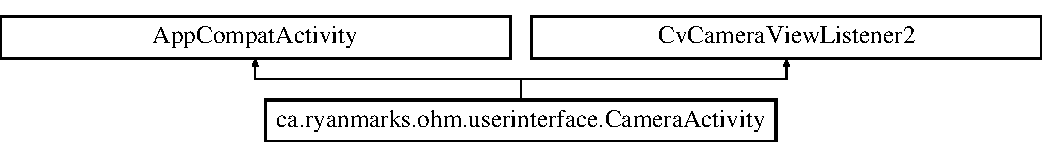
\includegraphics[height=1.911263cm]{classca_1_1ryanmarks_1_1ohm_1_1userinterface_1_1_camera_activity}
\end{center}
\end{figure}
\subsection*{Public Member Functions}
\begin{DoxyCompactItemize}
\item 
void \hyperlink{classca_1_1ryanmarks_1_1ohm_1_1userinterface_1_1_camera_activity_afa73d36e5322e895558c6663acb190bf}{on\+Create} (Bundle saved\+Instance\+State)
\item 
void \hyperlink{classca_1_1ryanmarks_1_1ohm_1_1userinterface_1_1_camera_activity_a34efe943c0d3769ad9b9f9866974836f}{on\+Pause} ()
\item 
void \hyperlink{classca_1_1ryanmarks_1_1ohm_1_1userinterface_1_1_camera_activity_a9178d308984ee4f944f051adc205373d}{on\+Resume} ()
\item 
\hypertarget{classca_1_1ryanmarks_1_1ohm_1_1userinterface_1_1_camera_activity_ada3e30d69cbb69ed1f34827cf20ca17d}{}\label{classca_1_1ryanmarks_1_1ohm_1_1userinterface_1_1_camera_activity_ada3e30d69cbb69ed1f34827cf20ca17d} 
void {\bfseries on\+Destroy} ()
\item 
void \hyperlink{classca_1_1ryanmarks_1_1ohm_1_1userinterface_1_1_camera_activity_a57e9b0251cfc888e8514a45f88bec4a4}{on\+Camera\+View\+Started} (int width, int height)
\item 
void \hyperlink{classca_1_1ryanmarks_1_1ohm_1_1userinterface_1_1_camera_activity_a33cb29ef55f85b3459231b01d15db6c3}{on\+Camera\+View\+Stopped} ()
\item 
Mat \hyperlink{classca_1_1ryanmarks_1_1ohm_1_1userinterface_1_1_camera_activity_a91c2f08d2f0fa30ee24c1c8420d0b420}{on\+Camera\+Frame} (Camera\+Bridge\+View\+Base.\+Cv\+Camera\+View\+Frame input\+Frame)
\end{DoxyCompactItemize}


\subsection{Member Function Documentation}
\hypertarget{classca_1_1ryanmarks_1_1ohm_1_1userinterface_1_1_camera_activity_a91c2f08d2f0fa30ee24c1c8420d0b420}{}\label{classca_1_1ryanmarks_1_1ohm_1_1userinterface_1_1_camera_activity_a91c2f08d2f0fa30ee24c1c8420d0b420} 
\index{ca\+::ryanmarks\+::ohm\+::userinterface\+::\+Camera\+Activity@{ca\+::ryanmarks\+::ohm\+::userinterface\+::\+Camera\+Activity}!on\+Camera\+Frame@{on\+Camera\+Frame}}
\index{on\+Camera\+Frame@{on\+Camera\+Frame}!ca\+::ryanmarks\+::ohm\+::userinterface\+::\+Camera\+Activity@{ca\+::ryanmarks\+::ohm\+::userinterface\+::\+Camera\+Activity}}
\subsubsection{\texorpdfstring{on\+Camera\+Frame()}{onCameraFrame()}}
{\footnotesize\ttfamily Mat ca.\+ryanmarks.\+ohm.\+userinterface.\+Camera\+Activity.\+on\+Camera\+Frame (\begin{DoxyParamCaption}\item[{Camera\+Bridge\+View\+Base.\+Cv\+Camera\+View\+Frame}]{input\+Frame }\end{DoxyParamCaption})}

This method performs the transformation from the acquired camera frame to the image that is shown to the user. It identifies resistances and overlays the resistance value 
\begin{DoxyParams}{Parameters}
{\em input\+Frame} & The camera frame captured \\
\hline
\end{DoxyParams}
\begin{DoxyReturn}{Returns}
The image to be shown to the user 
\end{DoxyReturn}
\hypertarget{classca_1_1ryanmarks_1_1ohm_1_1userinterface_1_1_camera_activity_a57e9b0251cfc888e8514a45f88bec4a4}{}\label{classca_1_1ryanmarks_1_1ohm_1_1userinterface_1_1_camera_activity_a57e9b0251cfc888e8514a45f88bec4a4} 
\index{ca\+::ryanmarks\+::ohm\+::userinterface\+::\+Camera\+Activity@{ca\+::ryanmarks\+::ohm\+::userinterface\+::\+Camera\+Activity}!on\+Camera\+View\+Started@{on\+Camera\+View\+Started}}
\index{on\+Camera\+View\+Started@{on\+Camera\+View\+Started}!ca\+::ryanmarks\+::ohm\+::userinterface\+::\+Camera\+Activity@{ca\+::ryanmarks\+::ohm\+::userinterface\+::\+Camera\+Activity}}
\subsubsection{\texorpdfstring{on\+Camera\+View\+Started()}{onCameraViewStarted()}}
{\footnotesize\ttfamily void ca.\+ryanmarks.\+ohm.\+userinterface.\+Camera\+Activity.\+on\+Camera\+View\+Started (\begin{DoxyParamCaption}\item[{int}]{width,  }\item[{int}]{height }\end{DoxyParamCaption})}

Unneeded interface method from open\+CV 
\begin{DoxyParams}{Parameters}
{\em width} & -\/ the width of the frames that will be delivered \\
\hline
{\em height} & -\/ the height of the frames that will be delivered \\
\hline
\end{DoxyParams}
\hypertarget{classca_1_1ryanmarks_1_1ohm_1_1userinterface_1_1_camera_activity_a33cb29ef55f85b3459231b01d15db6c3}{}\label{classca_1_1ryanmarks_1_1ohm_1_1userinterface_1_1_camera_activity_a33cb29ef55f85b3459231b01d15db6c3} 
\index{ca\+::ryanmarks\+::ohm\+::userinterface\+::\+Camera\+Activity@{ca\+::ryanmarks\+::ohm\+::userinterface\+::\+Camera\+Activity}!on\+Camera\+View\+Stopped@{on\+Camera\+View\+Stopped}}
\index{on\+Camera\+View\+Stopped@{on\+Camera\+View\+Stopped}!ca\+::ryanmarks\+::ohm\+::userinterface\+::\+Camera\+Activity@{ca\+::ryanmarks\+::ohm\+::userinterface\+::\+Camera\+Activity}}
\subsubsection{\texorpdfstring{on\+Camera\+View\+Stopped()}{onCameraViewStopped()}}
{\footnotesize\ttfamily void ca.\+ryanmarks.\+ohm.\+userinterface.\+Camera\+Activity.\+on\+Camera\+View\+Stopped (\begin{DoxyParamCaption}{ }\end{DoxyParamCaption})}

Unneeded interface method from open\+CV \hypertarget{classca_1_1ryanmarks_1_1ohm_1_1userinterface_1_1_camera_activity_afa73d36e5322e895558c6663acb190bf}{}\label{classca_1_1ryanmarks_1_1ohm_1_1userinterface_1_1_camera_activity_afa73d36e5322e895558c6663acb190bf} 
\index{ca\+::ryanmarks\+::ohm\+::userinterface\+::\+Camera\+Activity@{ca\+::ryanmarks\+::ohm\+::userinterface\+::\+Camera\+Activity}!on\+Create@{on\+Create}}
\index{on\+Create@{on\+Create}!ca\+::ryanmarks\+::ohm\+::userinterface\+::\+Camera\+Activity@{ca\+::ryanmarks\+::ohm\+::userinterface\+::\+Camera\+Activity}}
\subsubsection{\texorpdfstring{on\+Create()}{onCreate()}}
{\footnotesize\ttfamily void ca.\+ryanmarks.\+ohm.\+userinterface.\+Camera\+Activity.\+on\+Create (\begin{DoxyParamCaption}\item[{Bundle}]{saved\+Instance\+State }\end{DoxyParamCaption})}

Called when the activity is first created by Android. \hypertarget{classca_1_1ryanmarks_1_1ohm_1_1userinterface_1_1_camera_activity_a34efe943c0d3769ad9b9f9866974836f}{}\label{classca_1_1ryanmarks_1_1ohm_1_1userinterface_1_1_camera_activity_a34efe943c0d3769ad9b9f9866974836f} 
\index{ca\+::ryanmarks\+::ohm\+::userinterface\+::\+Camera\+Activity@{ca\+::ryanmarks\+::ohm\+::userinterface\+::\+Camera\+Activity}!on\+Pause@{on\+Pause}}
\index{on\+Pause@{on\+Pause}!ca\+::ryanmarks\+::ohm\+::userinterface\+::\+Camera\+Activity@{ca\+::ryanmarks\+::ohm\+::userinterface\+::\+Camera\+Activity}}
\subsubsection{\texorpdfstring{on\+Pause()}{onPause()}}
{\footnotesize\ttfamily void ca.\+ryanmarks.\+ohm.\+userinterface.\+Camera\+Activity.\+on\+Pause (\begin{DoxyParamCaption}{ }\end{DoxyParamCaption})}

Disable camera acquisition while the application is paused \hypertarget{classca_1_1ryanmarks_1_1ohm_1_1userinterface_1_1_camera_activity_a9178d308984ee4f944f051adc205373d}{}\label{classca_1_1ryanmarks_1_1ohm_1_1userinterface_1_1_camera_activity_a9178d308984ee4f944f051adc205373d} 
\index{ca\+::ryanmarks\+::ohm\+::userinterface\+::\+Camera\+Activity@{ca\+::ryanmarks\+::ohm\+::userinterface\+::\+Camera\+Activity}!on\+Resume@{on\+Resume}}
\index{on\+Resume@{on\+Resume}!ca\+::ryanmarks\+::ohm\+::userinterface\+::\+Camera\+Activity@{ca\+::ryanmarks\+::ohm\+::userinterface\+::\+Camera\+Activity}}
\subsubsection{\texorpdfstring{on\+Resume()}{onResume()}}
{\footnotesize\ttfamily void ca.\+ryanmarks.\+ohm.\+userinterface.\+Camera\+Activity.\+on\+Resume (\begin{DoxyParamCaption}{ }\end{DoxyParamCaption})}

Whenever the application resumes ensures opencv is loaded. 

The documentation for this class was generated from the following file\+:\begin{DoxyCompactItemize}
\item 
ca/ryanmarks/ohm/userinterface/Camera\+Activity.\+java\end{DoxyCompactItemize}

\hypertarget{classca_1_1ryanmarks_1_1ohm_1_1_pair}{}\section{ca.\+ryanmarks.\+ohm.\+Pair$<$ T, T1 $>$ Class Template Reference}
\label{classca_1_1ryanmarks_1_1ohm_1_1_pair}\index{ca.\+ryanmarks.\+ohm.\+Pair$<$ T, T1 $>$@{ca.\+ryanmarks.\+ohm.\+Pair$<$ T, T1 $>$}}


This class represents a generic key, value pair.  


\subsection*{Public Member Functions}
\begin{DoxyCompactItemize}
\item 
\hypertarget{classca_1_1ryanmarks_1_1ohm_1_1_pair_ac9da70a05dbdaf125538ef8523d38641}{}\label{classca_1_1ryanmarks_1_1ohm_1_1_pair_ac9da70a05dbdaf125538ef8523d38641} 
{\bfseries Pair} (T key, T1 val)
\item 
\hypertarget{classca_1_1ryanmarks_1_1ohm_1_1_pair_a3ecb02c2223f3d59b995dd51be8044cb}{}\label{classca_1_1ryanmarks_1_1ohm_1_1_pair_a3ecb02c2223f3d59b995dd51be8044cb} 
T {\bfseries get\+Key} ()
\item 
\hypertarget{classca_1_1ryanmarks_1_1ohm_1_1_pair_a1d63c726a56a010afc3e75a77a61205f}{}\label{classca_1_1ryanmarks_1_1ohm_1_1_pair_a1d63c726a56a010afc3e75a77a61205f} 
T1 {\bfseries get\+Value} ()
\end{DoxyCompactItemize}


\subsection{Detailed Description}
This class represents a generic key, value pair. 

\begin{DoxyAuthor}{Author}
Ryan Marks 
\end{DoxyAuthor}


The documentation for this class was generated from the following file\+:\begin{DoxyCompactItemize}
\item 
ca/ryanmarks/ohm/Pair.\+java\end{DoxyCompactItemize}

\hypertarget{enumca_1_1ryanmarks_1_1ohm_1_1valueidentification_1_1_resistor_colour}{}\section{ca.\+ryanmarks.\+ohm.\+valueidentification.\+Resistor\+Colour Enum Reference}
\label{enumca_1_1ryanmarks_1_1ohm_1_1valueidentification_1_1_resistor_colour}\index{ca.\+ryanmarks.\+ohm.\+valueidentification.\+Resistor\+Colour@{ca.\+ryanmarks.\+ohm.\+valueidentification.\+Resistor\+Colour}}


Enum containing all of the possible colours that a resistor can take on. Also features member functions used to map the colours of bands to values used in the calculation process.  


\subsection*{Public Member Functions}
\begin{DoxyCompactItemize}
\item 
\hyperlink{enumca_1_1ryanmarks_1_1ohm_1_1valueidentification_1_1_resistor_colour_acb42e95aa5bb7456ab3b527860b463a1}{Resistor\+Colour} (int v)
\end{DoxyCompactItemize}
\subsection*{Static Public Member Functions}
\begin{DoxyCompactItemize}
\item 
\hypertarget{enumca_1_1ryanmarks_1_1ohm_1_1valueidentification_1_1_resistor_colour_aa59a2846269caad5bcec5ba4bbd79936}{}\label{enumca_1_1ryanmarks_1_1ohm_1_1valueidentification_1_1_resistor_colour_aa59a2846269caad5bcec5ba4bbd79936} 
static void {\bfseries train\+NN} (Reader training\+Data)
\item 
static int \hyperlink{enumca_1_1ryanmarks_1_1ohm_1_1valueidentification_1_1_resistor_colour_a1f68c450e6879bce8909fca12402a1d7}{fit} (float r, float g, float b)
\item 
static int \hyperlink{enumca_1_1ryanmarks_1_1ohm_1_1valueidentification_1_1_resistor_colour_a26b7f5d2026cd9064a67ff6409c79562}{fit} (int r, int g, int b, int color\+Space)
\end{DoxyCompactItemize}
\subsection*{Public Attributes}
\begin{DoxyCompactItemize}
\item 
\hypertarget{enumca_1_1ryanmarks_1_1ohm_1_1valueidentification_1_1_resistor_colour_a4240e0fba2bf6534c36d80518a07b7a1}{}\label{enumca_1_1ryanmarks_1_1ohm_1_1valueidentification_1_1_resistor_colour_a4240e0fba2bf6534c36d80518a07b7a1} 
{\bfseries B\+L\+A\+CK} =(0)
\item 
\hypertarget{enumca_1_1ryanmarks_1_1ohm_1_1valueidentification_1_1_resistor_colour_a78a7455fa4bb58fc2c72fdfdc5a3c03f}{}\label{enumca_1_1ryanmarks_1_1ohm_1_1valueidentification_1_1_resistor_colour_a78a7455fa4bb58fc2c72fdfdc5a3c03f} 
{\bfseries B\+R\+O\+WN} =(1)
\item 
\hypertarget{enumca_1_1ryanmarks_1_1ohm_1_1valueidentification_1_1_resistor_colour_a0c1a0b300f5296355ab135cc124f4028}{}\label{enumca_1_1ryanmarks_1_1ohm_1_1valueidentification_1_1_resistor_colour_a0c1a0b300f5296355ab135cc124f4028} 
{\bfseries R\+ED} =(2)
\item 
\hypertarget{enumca_1_1ryanmarks_1_1ohm_1_1valueidentification_1_1_resistor_colour_ab4874691b468894f4bf6e1d40299b5a8}{}\label{enumca_1_1ryanmarks_1_1ohm_1_1valueidentification_1_1_resistor_colour_ab4874691b468894f4bf6e1d40299b5a8} 
{\bfseries O\+R\+A\+N\+GE} =(3)
\item 
\hypertarget{enumca_1_1ryanmarks_1_1ohm_1_1valueidentification_1_1_resistor_colour_a0bc011566bc76771fb4eef2a2b786c1b}{}\label{enumca_1_1ryanmarks_1_1ohm_1_1valueidentification_1_1_resistor_colour_a0bc011566bc76771fb4eef2a2b786c1b} 
{\bfseries Y\+E\+L\+L\+OW} =(4)
\item 
\hypertarget{enumca_1_1ryanmarks_1_1ohm_1_1valueidentification_1_1_resistor_colour_aa5ccc3e078be06cc66f94bde4cc3d555}{}\label{enumca_1_1ryanmarks_1_1ohm_1_1valueidentification_1_1_resistor_colour_aa5ccc3e078be06cc66f94bde4cc3d555} 
{\bfseries G\+R\+E\+EN} =(5)
\item 
\hypertarget{enumca_1_1ryanmarks_1_1ohm_1_1valueidentification_1_1_resistor_colour_a9b38ed752bd766a925f9e11488f23172}{}\label{enumca_1_1ryanmarks_1_1ohm_1_1valueidentification_1_1_resistor_colour_a9b38ed752bd766a925f9e11488f23172} 
{\bfseries B\+L\+UE} =(6)
\item 
\hypertarget{enumca_1_1ryanmarks_1_1ohm_1_1valueidentification_1_1_resistor_colour_a44829ddc544993ea4f1fa046b3c72674}{}\label{enumca_1_1ryanmarks_1_1ohm_1_1valueidentification_1_1_resistor_colour_a44829ddc544993ea4f1fa046b3c72674} 
{\bfseries V\+I\+O\+L\+ET} =(7)
\item 
\hypertarget{enumca_1_1ryanmarks_1_1ohm_1_1valueidentification_1_1_resistor_colour_a4687f14a4b02da9f4ed9fb1caef41e54}{}\label{enumca_1_1ryanmarks_1_1ohm_1_1valueidentification_1_1_resistor_colour_a4687f14a4b02da9f4ed9fb1caef41e54} 
{\bfseries G\+R\+EY} =(8)
\item 
\hypertarget{enumca_1_1ryanmarks_1_1ohm_1_1valueidentification_1_1_resistor_colour_a4001dd23d8298c409fc461064108b907}{}\label{enumca_1_1ryanmarks_1_1ohm_1_1valueidentification_1_1_resistor_colour_a4001dd23d8298c409fc461064108b907} 
{\bfseries W\+H\+I\+TE} =(9)
\item 
\hypertarget{enumca_1_1ryanmarks_1_1ohm_1_1valueidentification_1_1_resistor_colour_a35f511f90b6d2825f5f3cabc11ea73ec}{}\label{enumca_1_1ryanmarks_1_1ohm_1_1valueidentification_1_1_resistor_colour_a35f511f90b6d2825f5f3cabc11ea73ec} 
{\bfseries G\+O\+LD} =(11)
\item 
\hypertarget{enumca_1_1ryanmarks_1_1ohm_1_1valueidentification_1_1_resistor_colour_a0c64488768619664bc7f3cbda8edf1c6}{}\label{enumca_1_1ryanmarks_1_1ohm_1_1valueidentification_1_1_resistor_colour_a0c64488768619664bc7f3cbda8edf1c6} 
{\bfseries B\+A\+SE} =(10)
\item 
\hypertarget{enumca_1_1ryanmarks_1_1ohm_1_1valueidentification_1_1_resistor_colour_a02762e9bc4bf046c12de90eb839467f3}{}\label{enumca_1_1ryanmarks_1_1ohm_1_1valueidentification_1_1_resistor_colour_a02762e9bc4bf046c12de90eb839467f3} 
int {\bfseries value}
\end{DoxyCompactItemize}
\subsection*{Static Public Attributes}
\begin{DoxyCompactItemize}
\item 
\hypertarget{enumca_1_1ryanmarks_1_1ohm_1_1valueidentification_1_1_resistor_colour_a5570e0edc316280599bc2ccaf9911a1a}{}\label{enumca_1_1ryanmarks_1_1ohm_1_1valueidentification_1_1_resistor_colour_a5570e0edc316280599bc2ccaf9911a1a} 
static K\+Nearest {\bfseries K\+NN}
\item 
\hypertarget{enumca_1_1ryanmarks_1_1ohm_1_1valueidentification_1_1_resistor_colour_a7ee78df9947727ee94f64ae1e0d80472}{}\label{enumca_1_1ryanmarks_1_1ohm_1_1valueidentification_1_1_resistor_colour_a7ee78df9947727ee94f64ae1e0d80472} 
static D\+Trees {\bfseries dt}
\end{DoxyCompactItemize}


\subsection{Detailed Description}
Enum containing all of the possible colours that a resistor can take on. Also features member functions used to map the colours of bands to values used in the calculation process. 

\begin{DoxyAuthor}{Author}
Jonathan Brown 
\end{DoxyAuthor}


\subsection{Constructor \& Destructor Documentation}
\hypertarget{enumca_1_1ryanmarks_1_1ohm_1_1valueidentification_1_1_resistor_colour_acb42e95aa5bb7456ab3b527860b463a1}{}\label{enumca_1_1ryanmarks_1_1ohm_1_1valueidentification_1_1_resistor_colour_acb42e95aa5bb7456ab3b527860b463a1} 
\index{ca\+::ryanmarks\+::ohm\+::valueidentification\+::\+Resistor\+Colour@{ca\+::ryanmarks\+::ohm\+::valueidentification\+::\+Resistor\+Colour}!Resistor\+Colour@{Resistor\+Colour}}
\index{Resistor\+Colour@{Resistor\+Colour}!ca\+::ryanmarks\+::ohm\+::valueidentification\+::\+Resistor\+Colour@{ca\+::ryanmarks\+::ohm\+::valueidentification\+::\+Resistor\+Colour}}
\subsubsection{\texorpdfstring{Resistor\+Colour()}{ResistorColour()}}
{\footnotesize\ttfamily ca.\+ryanmarks.\+ohm.\+valueidentification.\+Resistor\+Colour.\+Resistor\+Colour (\begin{DoxyParamCaption}\item[{int}]{v }\end{DoxyParamCaption})}


\begin{DoxyParams}{Parameters}
{\em v} & The number represented by the colour in the calculation of the resistor\textquotesingle{}s ohmage. \\
\hline
\end{DoxyParams}


\subsection{Member Function Documentation}
\hypertarget{enumca_1_1ryanmarks_1_1ohm_1_1valueidentification_1_1_resistor_colour_a1f68c450e6879bce8909fca12402a1d7}{}\label{enumca_1_1ryanmarks_1_1ohm_1_1valueidentification_1_1_resistor_colour_a1f68c450e6879bce8909fca12402a1d7} 
\index{ca\+::ryanmarks\+::ohm\+::valueidentification\+::\+Resistor\+Colour@{ca\+::ryanmarks\+::ohm\+::valueidentification\+::\+Resistor\+Colour}!fit@{fit}}
\index{fit@{fit}!ca\+::ryanmarks\+::ohm\+::valueidentification\+::\+Resistor\+Colour@{ca\+::ryanmarks\+::ohm\+::valueidentification\+::\+Resistor\+Colour}}
\subsubsection{\texorpdfstring{fit()}{fit()}\hspace{0.1cm}{\footnotesize\ttfamily [1/2]}}
{\footnotesize\ttfamily static int ca.\+ryanmarks.\+ohm.\+valueidentification.\+Resistor\+Colour.\+fit (\begin{DoxyParamCaption}\item[{float}]{r,  }\item[{float}]{g,  }\item[{float}]{b }\end{DoxyParamCaption})\hspace{0.3cm}{\ttfamily [static]}}

Function takes in a sampled colour from the images and attempts to fit it to the closest known colour a resistor can possess. 
\begin{DoxyParams}{Parameters}
{\em r} & The red colour value of the colour to be fit. \\
\hline
{\em g} & The green colour value of the colour to be fit. \\
\hline
{\em b} & The blue colour value of the colour to be fit. \\
\hline
\end{DoxyParams}
\begin{DoxyReturn}{Returns}
The known colour that best represents the sampled colour. 
\end{DoxyReturn}
\hypertarget{enumca_1_1ryanmarks_1_1ohm_1_1valueidentification_1_1_resistor_colour_a26b7f5d2026cd9064a67ff6409c79562}{}\label{enumca_1_1ryanmarks_1_1ohm_1_1valueidentification_1_1_resistor_colour_a26b7f5d2026cd9064a67ff6409c79562} 
\index{ca\+::ryanmarks\+::ohm\+::valueidentification\+::\+Resistor\+Colour@{ca\+::ryanmarks\+::ohm\+::valueidentification\+::\+Resistor\+Colour}!fit@{fit}}
\index{fit@{fit}!ca\+::ryanmarks\+::ohm\+::valueidentification\+::\+Resistor\+Colour@{ca\+::ryanmarks\+::ohm\+::valueidentification\+::\+Resistor\+Colour}}
\subsubsection{\texorpdfstring{fit()}{fit()}\hspace{0.1cm}{\footnotesize\ttfamily [2/2]}}
{\footnotesize\ttfamily static int ca.\+ryanmarks.\+ohm.\+valueidentification.\+Resistor\+Colour.\+fit (\begin{DoxyParamCaption}\item[{int}]{r,  }\item[{int}]{g,  }\item[{int}]{b,  }\item[{int}]{color\+Space }\end{DoxyParamCaption})\hspace{0.3cm}{\ttfamily [static]}}

Function takes in a sampled colour from the images and attempts to fit it to the closest known colour a resistor can possess. Function takes in a sampled colour from the images and attempts to fit\+Old it to the closest known colour a resistor can possess. 
\begin{DoxyParams}{Parameters}
{\em r} & The red colour value of the colour to be fit\+Old. \\
\hline
{\em g} & The green colour value of the colour to be fit\+Old. \\
\hline
{\em b} & The blue colour value of the colour to be fit\+Old. \\
\hline
\end{DoxyParams}
\begin{DoxyReturn}{Returns}
The known colour that best represents the sampled colour. 
\end{DoxyReturn}


The documentation for this enum was generated from the following file\+:\begin{DoxyCompactItemize}
\item 
ca/ryanmarks/ohm/valueidentification/Resistor\+Colour.\+java\end{DoxyCompactItemize}

\hypertarget{classca_1_1ryanmarks_1_1ohm_1_1input_1_1_scanning_camera_view}{}\section{ca.\+ryanmarks.\+ohm.\+input.\+Scanning\+Camera\+View Class Reference}
\label{classca_1_1ryanmarks_1_1ohm_1_1input_1_1_scanning_camera_view}\index{ca.\+ryanmarks.\+ohm.\+input.\+Scanning\+Camera\+View@{ca.\+ryanmarks.\+ohm.\+input.\+Scanning\+Camera\+View}}
Inheritance diagram for ca.\+ryanmarks.\+ohm.\+input.\+Scanning\+Camera\+View\+:\begin{figure}[H]
\begin{center}
\leavevmode
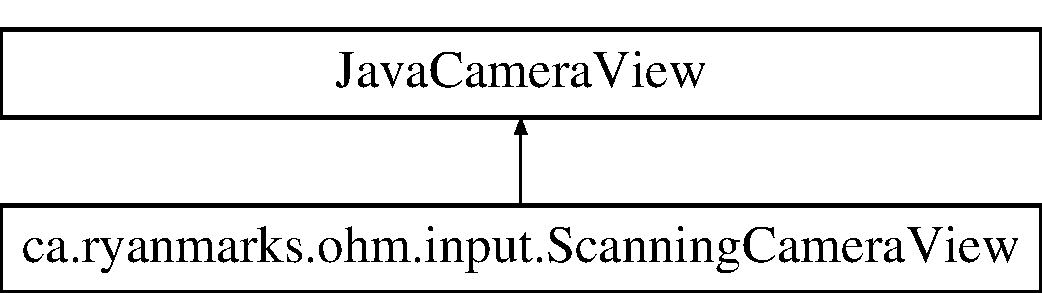
\includegraphics[height=2.000000cm]{classca_1_1ryanmarks_1_1ohm_1_1input_1_1_scanning_camera_view}
\end{center}
\end{figure}
\subsection*{Public Member Functions}
\begin{DoxyCompactItemize}
\item 
\hypertarget{classca_1_1ryanmarks_1_1ohm_1_1input_1_1_scanning_camera_view_ac0f86fb041db0384361798ae08a78853}{}\label{classca_1_1ryanmarks_1_1ohm_1_1input_1_1_scanning_camera_view_ac0f86fb041db0384361798ae08a78853} 
{\bfseries Scanning\+Camera\+View} (Context context, int camera\+Id)
\item 
\hypertarget{classca_1_1ryanmarks_1_1ohm_1_1input_1_1_scanning_camera_view_a723d3439c32c6060135610e6c744cb38}{}\label{classca_1_1ryanmarks_1_1ohm_1_1input_1_1_scanning_camera_view_a723d3439c32c6060135610e6c744cb38} 
{\bfseries Scanning\+Camera\+View} (Context context, Attribute\+Set attrs)
\end{DoxyCompactItemize}
\subsection*{Protected Member Functions}
\begin{DoxyCompactItemize}
\item 
boolean \hyperlink{classca_1_1ryanmarks_1_1ohm_1_1input_1_1_scanning_camera_view_a6a040425f2dd892fd5b81767203b405c}{initialize\+Camera} (int width, int height)
\end{DoxyCompactItemize}


\subsection{Member Function Documentation}
\hypertarget{classca_1_1ryanmarks_1_1ohm_1_1input_1_1_scanning_camera_view_a6a040425f2dd892fd5b81767203b405c}{}\label{classca_1_1ryanmarks_1_1ohm_1_1input_1_1_scanning_camera_view_a6a040425f2dd892fd5b81767203b405c} 
\index{ca\+::ryanmarks\+::ohm\+::input\+::\+Scanning\+Camera\+View@{ca\+::ryanmarks\+::ohm\+::input\+::\+Scanning\+Camera\+View}!initialize\+Camera@{initialize\+Camera}}
\index{initialize\+Camera@{initialize\+Camera}!ca\+::ryanmarks\+::ohm\+::input\+::\+Scanning\+Camera\+View@{ca\+::ryanmarks\+::ohm\+::input\+::\+Scanning\+Camera\+View}}
\subsubsection{\texorpdfstring{initialize\+Camera()}{initializeCamera()}}
{\footnotesize\ttfamily boolean ca.\+ryanmarks.\+ohm.\+input.\+Scanning\+Camera\+View.\+initialize\+Camera (\begin{DoxyParamCaption}\item[{int}]{width,  }\item[{int}]{height }\end{DoxyParamCaption})\hspace{0.3cm}{\ttfamily [protected]}}

Initialize a camera with the preferred parameters for resistor scanning 
\begin{DoxyParams}{Parameters}
{\em width} & the width of the pictures, in pixels \\
\hline
{\em height} & the height of the pictures, in pixels \\
\hline
\end{DoxyParams}
\begin{DoxyReturn}{Returns}
The success of the initialization 
\end{DoxyReturn}


The documentation for this class was generated from the following file\+:\begin{DoxyCompactItemize}
\item 
ca/ryanmarks/ohm/input/Scanning\+Camera\+View.\+java\end{DoxyCompactItemize}

\hypertarget{classca_1_1ryanmarks_1_1ohm_1_1valueidentification_1_1_value_calculator}{}\section{ca.\+ryanmarks.\+ohm.\+valueidentification.\+Value\+Calculator Class Reference}
\label{classca_1_1ryanmarks_1_1ohm_1_1valueidentification_1_1_value_calculator}\index{ca.\+ryanmarks.\+ohm.\+valueidentification.\+Value\+Calculator@{ca.\+ryanmarks.\+ohm.\+valueidentification.\+Value\+Calculator}}


Object used to calculate the resistance of the resistor based on the mapped colours.  


\subsection*{Public Member Functions}
\begin{DoxyCompactItemize}
\item 
\hypertarget{classca_1_1ryanmarks_1_1ohm_1_1valueidentification_1_1_value_calculator_a6221d53a82179e4f00298b47ba9af971}{}\label{classca_1_1ryanmarks_1_1ohm_1_1valueidentification_1_1_value_calculator_a6221d53a82179e4f00298b47ba9af971} 
{\bfseries Value\+Calculator} (Integer a, Integer b, Integer c, Integer d)
\item 
\hypertarget{classca_1_1ryanmarks_1_1ohm_1_1valueidentification_1_1_value_calculator_a9f276e3ead16c49bf1c291cf9facebb5}{}\label{classca_1_1ryanmarks_1_1ohm_1_1valueidentification_1_1_value_calculator_a9f276e3ead16c49bf1c291cf9facebb5} 
String {\bfseries get\+Value} ()
\end{DoxyCompactItemize}


\subsection{Detailed Description}
Object used to calculate the resistance of the resistor based on the mapped colours. 

\begin{DoxyAuthor}{Author}
Jonathan Brown 
\end{DoxyAuthor}


The documentation for this class was generated from the following file\+:\begin{DoxyCompactItemize}
\item 
ca/ryanmarks/ohm/valueidentification/Value\+Calculator.\+java\end{DoxyCompactItemize}

%--- End generated contents ---

% Index
\backmatter
\newpage
\phantomsection
\clearemptydoublepage
\addcontentsline{toc}{chapter}{Index}
\printindex

\end{document}
